%%%%%%%%%%%%%%%%%%%%%%% file template.tex %%%%%%%%%%%%%%%%%%%%%%%%%
%
% This is a general template file for the LaTeX package SVJour3
% for Springer journals.          Springer Heidelberg 2010/09/16
%
% Copy it to a new file with a new name and use it as the basis
% for your article. Delete % signs as needed.
%
% This template includes a few options for different layouts and
% content for various journals. Please consult a previous issue of
% your journal as needed.
%
%%%%%%%%%%%%%%%%%%%%%%%%%%%%%%%%%%%%%%%%%%%%%%%%%%%%%%%%%%%%%%%%%%%
%
% First comes an example EPS file -- just ignore it and
% proceed on the \documentclass line
% your LaTeX will extract the file if required
% \begin{filecontents*}{example.eps}
% %!PS-Adobe-3.0 EPSF-3.0
% %%BoundingBox: 19 19 221 221
% %%CreationDate: Mon Sep 29 1997
% %%Creator: programmed by hand (JK)
% %%EndComments
% gsave
% newpath
%   20 20 moveto
%   20 220 lineto
%   220 220 lineto
%   220 20 lineto
% closepath
% 2 setlinewidth
% gsave
%   .4 setgray fill
% grestore
% stroke
% grestore
% \end{filecontents*}
%
\RequirePackage{fix-cm}
%
%\documentclass{svjour3}                     % onecolumn (standard format)
%\documentclass[smallcondensed]{svjour3}     % onecolumn (ditto)
\documentclass[smallextended]{svjour3}       % onecolumn (second format)
%\documentclass[twocolumn]{svjour3}          % twocolumn
%
\smartqed  % flush right qed marks, e.g. at end of proof
%
\usepackage{booktabs}
\usepackage{graphicx}
\usepackage{times}
\usepackage{latexsym,mathrsfs}
\usepackage{amssymb,amsfonts,amsmath}
\usepackage[numbers]{natbib}
% \usepackage{algorithm}
% \usepackage{algpseudocode}
% \usepackage{algorithmicx}
\usepackage{color}
\usepackage{graphics}
\usepackage{graphicx}
\usepackage{bbm}
\usepackage{url}
\def\ds{\displaystyle}
\def\R{\mathbb{R}}
\newcommand{\x}{\mathbf{x}}
\newcommand{\X}{\mathbf{X}}
\newcommand{\y}{\mathbf{y}}
\newcommand{\f}{\mathbf{f}}
\newcommand{\Y}{\mathbf{Y}}
\newcommand{\F}{\mathbf{F}}
\newcommand{\z}{\mathbf{z}}
\newcommand{\s}{\mathbf{x}}
\newcommand{\Sset}{\mathbb{X}}
\newcommand{\Rset}{\mathbb{R}}
\newcommand{\Xset}{\mathbb{X}}
\newcommand{\Prob}{\mathbb{P}}

% packages and dependencies for colored comments in text (collab_tex is the package, the other ones are dependencies)
\usepackage[dvipsnames,svgnames]{xcolor}
\usepackage[normalem]{ulem}
\usepackage{collab_tex}

\begin{document}

\title{Warping%\thanks{Grants or other notes
%about the article that should go on the front page should be
%placed here. General acknowledgments should be placed at the end of the article.}
}

%\titlerunning{Short form of title}        % if too long for running head

\author{Victor Picheny         \and
        Coralie Picard        \and
        Gael Thebaud
}

%\authorrunning{Short form of author list} % if too long for running head

\institute{V. Picheny \at
              MIAT, Universit\'e de Toulouse, INRA, Castanet-Tolosan, France \\
              Tel.:  +33561285551\\
              \email{victor.picheny@inra.fr}           %  \\
%             \emph{Present address:} of F. Author  %  if needed
\and
           C. Picard \at
           BGPI, Montpellier SupAgro, INRA, Univ. Montpellier, Cirad, TA A-54/K, 34398, Montpellier 
           \and
           G. Thebaud \at to do
}

\date{Received: date / Accepted: date}
% The correct dates will be entered by the editor

\maketitle

\begin{abstract}
On peut \victor{faire un commentaire} \coralie{chacun avec sa couleur}, on peut aussi \victordelete{enlever des trucs} ou bien \coralieadd{ajouter d'autres trucs}, \gaeladd{et Gael aussi}.
\keywords{to do}
\end{abstract}

\section{Introduction}
\victor{toi ou moi}
Mathematical modelling for design, in particular in epidemiology

\victor{pour toi... mais peut-être plus facile à faire une fois que le reste aura avancé}

The sharka model and objectives

\victor{le reste de l'intro pour moi}

Generalities on optimization

Bayesian optimization

Problem at hand: dealing with local invariances

Outline

\section{Model description and problem set-up}
\victor{Section à remplir par toi ! Suggestion de plan détaillé.}

What does it model

How the model works

What problem do we want to solve

Inputs description

Invariances descriptions

Table of inputs with range of variation

Table of invariance relations
\\

The simulation model that we analyze in this work is a stochastic, spatially explicit, SEIR (susceptible-exposed-infectious-removed) model that simulates sharka spread and management actions (including surveillance, removals and replantations, Pleydell et al. 2018; Rimbaud et al. 2018a, 2018b).
This model is orchard-based, with a discrete time step of one week. It allows to perform simulations on landscapes composed of uncultivated areas and patches on which peach trees are grown. The patches can be more or less aggregated in the landscape however, we only use the landscapes with a high patch aggregation as described by Picard et al. 2018. During the simulation, the trees in the patches are characterized by different states. When the simulation begins, they are not infected: they are in the “susceptible” state. Then, the virus is introduced the first year of the simulation in one of the patches and spreads through orchards, causing changes in tree status: from “susceptible”, they become “exposed” (infected but not yet infectious or symptomatic), “infectious hidden” (after the end of the latent period), “infectious detected” (when specific symptoms are detected on the tree during a survey), and "removed" (when the tree is removed from the patch). In addition, new introductions can also occur during the entire simulation on all patches.
The model output is an economic criterion, the net present value (NPV), which accounts for the benefit generated by the cultivation of productive trees and the costs induced by fruit production and disease management (Rimbaud et al. 2018b).
In addition, in order to simulate wide range of epidemic and management scenarios, the model includes 6 epidemiological and 23 management parameters (Rimbaud et al. 2018b, Picard et al. 2018). In this work, we will use the 6 epidemiological parameters and only 10 management parameters (related to the surveillance of the orchards). They include distances of 3 zones for which the surveys are more or less frequent as well as their duration, the probability of the infected tree detection, and a contamination threshold which can request to improve the surveillance frequency in the focal zone. Details of epidemiological and management parameters used in this study are presented in Fig.\ref{fig:schemagestion} and Table \ref{tab:tableparameters} (this table also includes their variation ranges in the model).

Here, the purpose is to optimize the management strategy of the disease (i.e. to find the combination of management parameters allowing to obtain the best NPV), taking into account the epidemic stochasticity. However, we note that some combinations of management parameters can represent the same management, which may cause problems in the optimization process. Indeed, we observe that some management parameters are not useful when others parameters are assigned a value of 0, which means that they can take any values without modifying the simulation. For example, when a zone radius is 0, the associated surveillance frequencies have no impact on the NPV regardless the radius value. The methodological developments that are proposed in this work address this issue by removing the parameter combinations which lead to the same management. The parameter invariances removed are listed in Table \ref{tab:table_invariances_parameters}.


% Table paras de gestion
\begin{table}[htbp]
	\centering
	\caption{Epidemiological and management parameters implemented in the previously developed model  with minimum and maximum values corresponding to the variation range of each parameter.}
	\begin{tabular}{|c|p{33.785em}|c|c|}
		\cmidrule{3-4}    \multicolumn{1}{c}{} & \multicolumn{1}{c|}{} & \textbf{Min} & \textbf{Max} \\
		\midrule
		\multicolumn{4}{|c|}{\textbf{Epidemiological parameters}} \\
		\midrule
		$q_{K}$    & Quantile of the connectivity of the patch of first introduction & 0     & 1 \\
		\midrule
		$\phi$ & Probability of introduction at plantation (before management) & 0,02  & 0,02 \\
		\cmidrule{2-4}          & Probability of introduction at plantation (during management) & 0,0046 & 0,0107 \\
		\midrule
		$p_{MI}$ & Relative probability of massive introduction (before management) & 0,4   & 0,4 \\
		\cmidrule{2-4}          & Relative probability of massive introduction  (during management) & 0     & 0,1 \\
		\midrule
		$W_{exp}$  & Expected value of the dispersal weighting variable & 0,469 & 0,504 \\
		\midrule
		$\beta$     & Transmission coefficient & 1,25  & 1,39 \\
		\midrule
		$\theta_{exp}$  & Variance of the latent period duration (years) & 1,71  & 2,14 \\
		\midrule
		\multicolumn{4}{|c|}{\textbf{Management parameters}} \\
		\midrule
		$\rho$    & Probability of detection of a symptomatic tree & 0     & 0,66 \\
		\midrule
		$\gamma_{O}$    & Duration of observation zones (years) & 0     & 10 \\
		\midrule
		$\zeta_{s}$   & Radius-distance of security zones (m) & 0     & 5800 \\
		\midrule
		$\zeta_{f}$  & Radius-distance of focal zones (m) & 0     & 1 \\
		\midrule
		$\zeta_{eO}$ & Radius-distance of observation epicenter (m) & 0     & 1 \\
		\midrule
		1/$\eta_{0}$  & Maximal period between 2 observations (year) & 1     & 15 \\
		\midrule
		$\eta_{s}$    & Observation frequency in security zones (year-1) & 0     & 8 \\
		\midrule
		$\eta_{f}$    & Observation frequency in focal zones (year-1) & 0     & 8 \\
		\midrule
		$\eta_{f*}$   & Modified observation frequency in focal zones (year-1) & 0     & 8 \\
		\midrule
		$\chi_{o}$    & Contamination threshold in the observation epicenter, above which the observation frequency in focal zone is modified & 0     & 1 \\
		\bottomrule
	\end{tabular}%
	\label{tab:tableparameters}%
\end{table}%

\begin{figure}[!ht]
	\centering
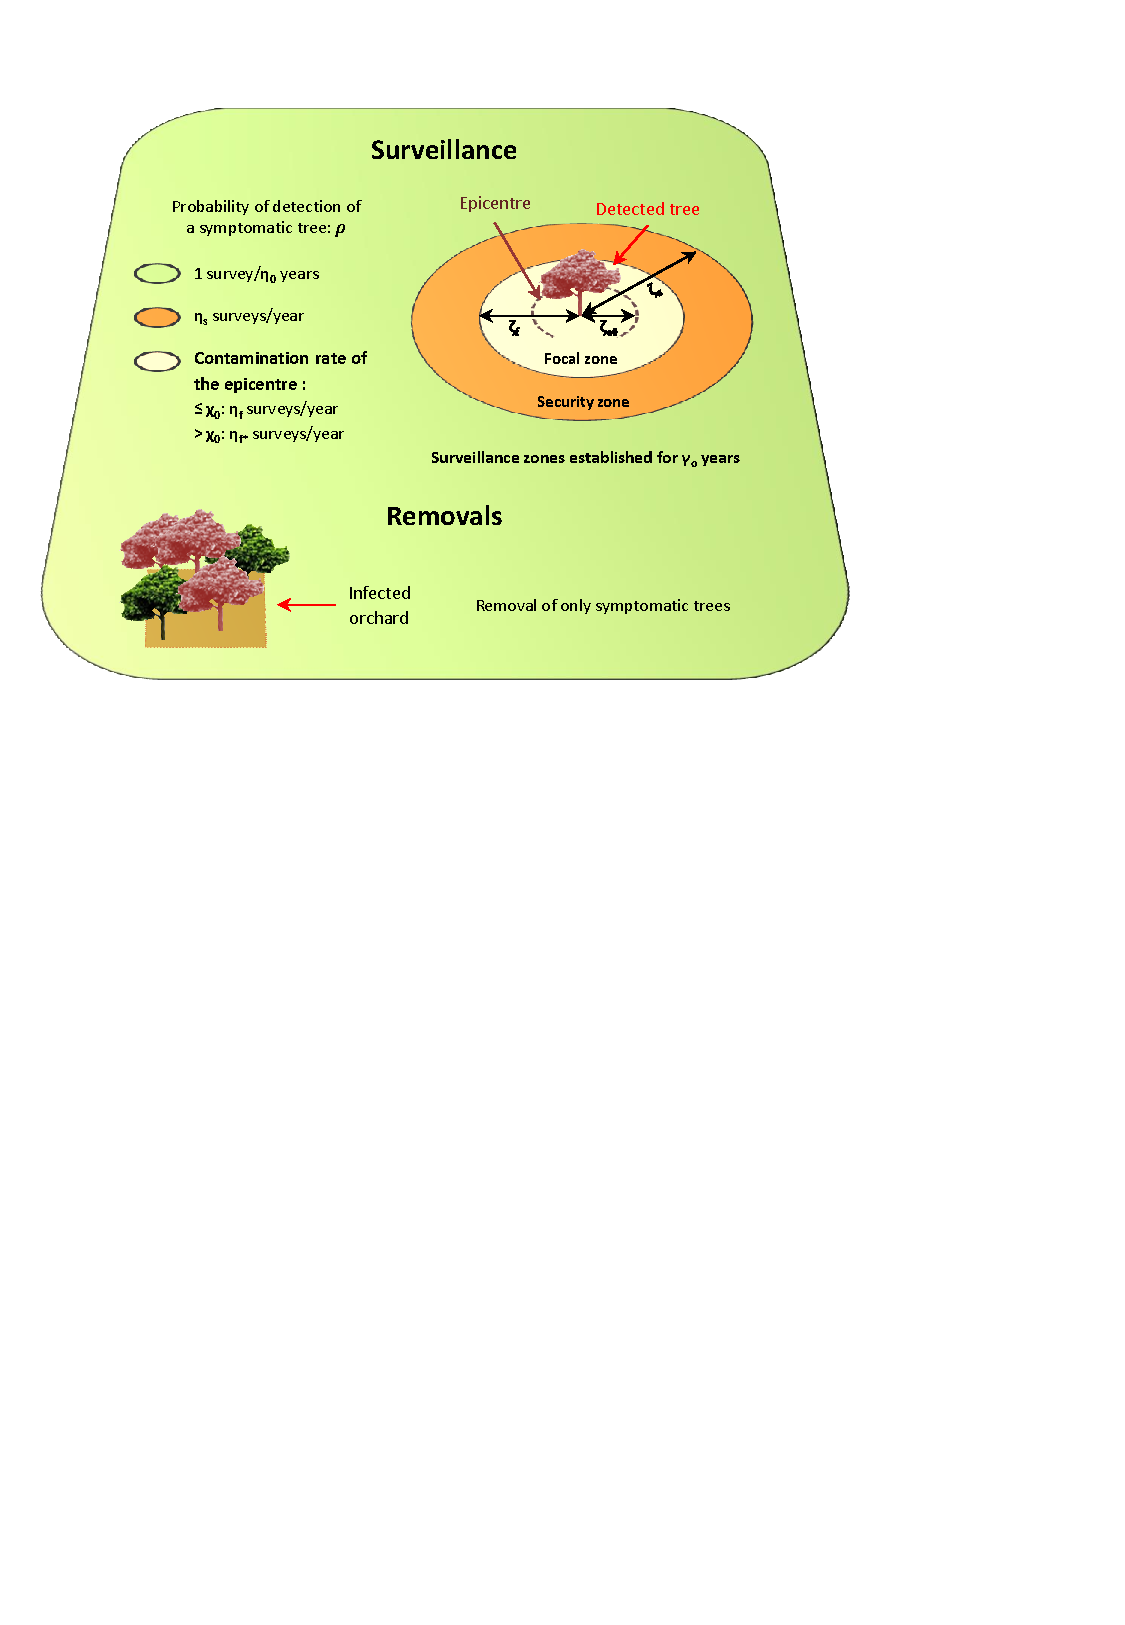
\includegraphics[trim = 0cm 16cm 4cm 1cm, clip]{Figures_Warping_paras_de_gestion.pdf}
 \caption{Management actions implemented in the model}\label{fig:schemagestion}
\end{figure}

% Table invariances paras de gestion
\begin{table}[htbp]
	\centering
	\caption{Invariances of management parameters}
	\begin{tabular}{|c|c|c|c|c|}
		\midrule
		\textbf{Warping} & \textbf{Management parameters} & \textbf{OR} & \textbf{OR} & \textbf{OR} \\
		\midrule
		\textbf{No warping} & $\rho$ & & & \\
		\cmidrule{2-5} & 1/$\eta_{0}$ & & & \\
		\cmidrule{2-5} & $\gamma_{O}$ & & & \\
		\midrule
		\textbf{Warping based on warped variables} & $\chi_{o}$ & $\gamma_{O}$ = 0 & $\rho$ = 0 & \\
		\cmidrule{2-5} & $\zeta_{eO}$ & $\gamma_{O}$ = 0 & $\zeta_{s}$ = 0 & $\rho$ = 0\\
		\cmidrule{2-5} & $\zeta_{f}$ & $\gamma_{O}$ = 0 & $\zeta_{s}$ = 0 & \\
		\midrule
		\textbf{Circular conditions} & $\eta_{f*}$ & $\gamma_{O}$ = 0 & $\rho$ = 0 & \\
		\cmidrule{2-5} & $\zeta_{s}$ & $\gamma_{O}$ = 0 & $\eta_{s}$ = 0 & \\
		\cmidrule{2-5} & $\eta_{s}$ & $\gamma_{O}$ = 0 & & \\
		\cmidrule{2-5} & $\eta_{f}$ & $\gamma_{O}$ = 0 & & \\
		\midrule

	\end{tabular}%
	\label{tab:table_invariances_parameters}%
\end{table}%


\section{Methods — Bayesian optimization}

\subsection{Overview}

\subsection{Bayesian optimization of stochastic simulators}

\subsection{Bayesian optimization with invariances}

\subsubsection{Definitions}

\subsubsection{Simple warping}

\subsubsection{Warping based on linear relations}

\subsubsection{Combining warpings}

\section{Experiments on toy problems}

\subsection{Problem descriptions}

\subsection{Comparison metrics}

\subsection{Results}

\section{A warping-based Bayesian optimization of the Sharka model}

\subsection{Numerical setup}

\subsubsection{Experiments description}

\victor{Premier jet par toi ?}

\subsubsection{Comparison with standard BO}

Description of comparison metrics

\victor{Idem juste pour les méthodes de comparaison, je me charge du paragraphe pour dire à quoi on se compare et je m'occupe de la partie krigeage et warping.}

\subsection{Results and insights into the Sharka model}

\section{Conclusion}

What we did (the problem we solved)

What we proposed: warping to tackle invariances. Proof of concept

Possible extensions

\section*{References}
\end{document}